%%%%%%%%%%%%%%%%%%%%%%%%%%%%%%%%%%%%%%%%%%%%%%%%%%%%%%
\documentclass[11pt]{article}
%%%%%%%%%%%%%%%%%%%%%%%%%%%%%%%%%%%%%%%%%%%%%%%%%%%%%%

\usepackage{amsmath}
\usepackage{amsthm}
\usepackage{amssymb}
\usepackage{latexsym}
\usepackage{graphicx}
\usepackage{color}
\usepackage{verbatim}
\usepackage{float}
\usepackage{multicol}
\usepackage{xcolor}
\usepackage{listings}
\usepackage{tikz}
\usetikzlibrary{arrows.meta, positioning, calc}
\usetikzlibrary{decorations.pathmorphing}
\usepackage{tcolorbox}
\tcbuselibrary{breakable}
\usepackage{cancel}


\newtcolorbox{solutionbox}{
  breakable,
  colback=blue!5!white,
  colframe=blue!50!black,
  title=Solution,
  sharp corners,
  boxrule=0.8pt
}

\newtcolorbox{hintbox}{
  breakable,
  colback=gray!10!white,
  colframe=gray!50!black,
  title=Hint,
  sharp corners,
  boxrule=0.5pt
}

% Unnumbered theorem
\newtheorem*{thm*}{Theorem}

\lstdefinelanguage{R}{
      keywords={if,else,while,for,in,next,break,function,TRUE,FALSE,NULL,Inf,NA,NaN,switch,repeat,return,require,library},
      keywordstyle=\color{blue}\bfseries,
      identifierstyle=\color{black},
      comment=[l]{\#},
      commentstyle=\color{gray}\ttfamily,
      string=[b]{"},
      stringstyle=\color{red}\ttfamily,
      morecomment=[l]{//},
      morestring=[b]{'},
      sensitive=true,
      morekeywords={print,summary,plot,lm,glm,data,frame,read.csv,write.csv,factor,levels,names,colnames,rownames,
      head,tail,str,dim,length,class,typeof,mode,is.na,is.null,is.finite,is.infinite,is.nan,as.numeric,as.character,
      as.factor,as.Date,as.POSIXct,as.matrix,as.data.frame,rbind,cbind,merge,subset,aggregate,tapply,apply,lapply,sapply,
      mapply,vapply,replicate,seq,rep,c,list,matrix,array,data.frame,table,hist,boxplot,barplot,pie,curve,lines,points,text,
      abline,legend,par,mtext,title,xlab,ylab,xlim,ylim,main,sub,col,pch,cex,lty,lwd,type,bg,fg,args,options,warnings,errors,
      message,stop,warning,error,try,tryCatch,withCallingHandlers,on.exit,debug,browser,trace,recover,options,getOption,setOption},
    }


\setlength{\textheight}{9in}
\setlength{\textwidth}{6in}
\addtolength{\topmargin}{-2cm}
\addtolength{\oddsidemargin}{-1cm}
\parindent=0in


\def\classnum{3810}
\def\classtitle{Probability}
\def\classtitleshort{Probability}
\def\classsec{001}
\def\classterm{Fall 2025}
\def\instructor{Robert Rostermundt}
%\def\hmwknum{\#2}


%%%%%%%%%%%%%%%%%%%%%%%%%%%%%%%%%%%%%%%%%%%%%%%%%%%%%%%%%
%%%%%%%%%%%%%%%%%%%%%%%%%  Colors  %%%%%%%%%%%%%%%%%%%%%%
%%%%%%%%%%%%%%%%%%%%%%%%%%%%%%%%%%%%%%%%%%%%%%%%%%%%%%%%%

\definecolor{Green}{rgb}{0,.5,0}
%use for definitions
\definecolor{Red}{rgb}{.8,.2,0}
%use for emphasis
\definecolor{Yellow}{rgb}{.6,.6,.1}
%use for part titles
\definecolor{Cyan}{rgb}{.2,.6,.7}
%use for comments
\definecolor{Purple}{rgb}{.4,0,1}
%use for examples
\definecolor{deepred}{rgb}{.53,.29,.24}
%use for important points
\definecolor{Black}{rgb}{0,0,0}
%use for washout
\definecolor{Grey}{rgb}{.45,.45,.45}
% use for theorems
\newcommand{\tred}[1]{\textcolor{Red}{#1}}
\newcommand{\tgreen}[1]{\textcolor{Green}{#1}}
\newcommand{\tcyan}[1]{\textcolor{Cyan}{#1}}
\newcommand{\tyellow}[1]{\textcolor{Yellow}{#1}}
\newcommand{\tpurple}[1]{\textcolor{Purple}{#1}}
\newcommand{\tblack}[1]{\textcolor{Black}{#1}}
\newcommand{\tgrey}[1]{\textcolor{Grey}{#1}}
\newcommand{\tdeepred}[1]{\textcolor{deepred}{#1}}
\newcommand{\ttt}[1]{\texttt{#1}}

%%%%%%%%%%%%%%%%%%%%%%%%%%%%%%%%%%%%%%%%%%%%%%%%%%%%%%%%%
%%%%%%%%%%%%%%%%%%%%%%%%%  Theorem Environments  %%%%%%%%
%%%%%%%%%%%%%%%%%%%%%%%%%%%%%%%%%%%%%%%%%%%%%%%%%%%%%%%%%

\theoremstyle{plain}
\newtheorem{thm}{Theorem}
\newtheorem{axiom}{Axiom}
\newtheorem{cor}{Corollary}
\newtheorem{lemma}{Lemma}
\newtheorem{prop}{Proposition}
\newtheorem{ques}{Question}
\theoremstyle{definition}
\newtheorem{defn}{Definition}
\theoremstyle{remark}
\newtheorem{remark}{Remark}
\theoremstyle{definition}
\newtheorem{ex}{Example}
\numberwithin{equation}{section}
\newtheorem{prob}{Problem}
\numberwithin{equation}{section}


%%%%%%%%%%%%%%%%%%%%%%%%%%%%%%%%%%%%%%%%%%%%%%%%%%%%%%%%%
%%%%%%%%%%%%%%%%%%%%%%%%%  Math    %%%%%%%%%%%%%%%%%%%%%%
%%%%%%%%%%%%%%%%%%%%%%%%%%%%%%%%%%%%%%%%%%%%%%%%%%%%%%%%%


\newcommand{\abs}[1]{\left\lvert{#1}\right\rvert}
\newcommand{\card}[1]{\lvert{#1}\rvert}
\newcommand{\union}{\cup}
\newcommand{\Union}{\bigcup}
\newcommand{\inter}{\cap}
\newcommand{\Inter}{\bigcap}
%\newcommand{\hint}[1]{\medskip\newline\emph{Hint: #1}}
%\newcommand{\note}[1]{\medskip\newline\emph{Note: #1}}
\newcommand{\points}[1]{[#1 points]}
\newcommand{\totalpoints}[1]{[#1 points total]}
\newcommand{\ds}{\displaystyle}
\newcommand{\ben}{\begin{enumerate}}
\newcommand{\een}{\end{enumerate}}
\newcommand{\bi}{\begin{itemize}}
\newcommand{\ei}{\end{itemize}}
\newcommand{\beq}{\begin{eqnarray*}}
\newcommand{\eeq}{\end{eqnarray*}}
\newcommand{\bieq}{\begin{IEEEeqnarray}{rCl}}
\newcommand{\bieqx}{\begin{IEEEeqnarray}{+rCl+x*}}
\newcommand{\eieq}{\end{IEEEeqnarray}}
\newcommand{\nn}{\nonumber}
%\renewcommand{\i}{\item}
\newcommand{\bpm}{\begin{pmatrix}}
\newcommand{\epm}{\end{pmatrix}}
\newcommand{\sol}{\indent{\bf\emph{Solution:}}}
\newcommand{\ssol}{\indent{\\[2mm]\bf\emph{Solution:}}\;}
\newcommand{\hint}{\indent{\bf\emph{Hint}:}\;}
\newcommand{\note}{\indent{\bf\emph{Note}:}\;}
\newcommand{\vsk}{\vskip 2mm}
%%%%%%%%%%%%%%%%%%%%%%%%% Calculus %%%%%%%%%%%%%%%%%%%%%%%%%%%%
\newcommand{\dd}[2]{\ds\frac{d}{d{#1}}\left[{#2}\right]}
\newcommand{\der}[2]{\ds\frac{d{#1}}{d{#2}}}
\newcommand{\lmt}[3]{\ds\lim_{{#1}\to{#2}}{#3}}
\renewcommand{\iint}[2]{\ds\int{#1}\,d{#2}}
\newcommand{\dint}[4]{\ds\int^{#4}_{#3}{#1}\,d{#2}}
\renewcommand{\Delta}{\triangle}
%%%%%%%%%%%%%%%%%%%%%%%%% Number Sets %%%%%%%%%%%%%%%%%%%%%%%%%%
\newcommand{\N}{\mathbb{N}}
\newcommand{\Z}{\mathbb{Z}}
\newcommand{\Q}{\mathbb{Q}}
\newcommand{\R}{\mathbb{R}}
\newcommand{\C}{\mathbb{C}}
\newcommand{\F}{\mathcal{F}}
\renewcommand{\P}{\mathbb{P}}
\newcommand{\E}{\mathcal{E}}
\renewcommand{\o}{\omega}
\renewcommand{\O}{\Omega}
%%%%%%%%%%%%%%%%%%%%%%%%% Vectors %%%%%%%%%%%%%%%%%%%%%%%%%%%%%
\newcommand{\x}{\bar{x}}
\renewcommand{\v}{\bar{v}}
\newcommand{\y}{\bar{y}}
\newcommand{\z}{\bar{z}}
\newcommand{\w}{\bar{w}}
\renewcommand{\u}{\bar{u}}
\renewcommand{\b}{\bar{b}}
\newcommand{\e}{\bar{e}}
\renewcommand{\a}{\vec{a}}
\renewcommand{\r}{\vec{r}}
\newcommand{\vv}{\vec{v}}
\newcommand{\vecPQ}[2]{\overrightarrow{#1}{#2}}
\newcommand{\vecV}[1]{\overrightarrow{#1}}
\newcommand{\la}{\langle}
\newcommand{\ra}{\rangle}
%%%%%%%%%%%%%%%%%%%%%%%%%%% Vector Spaces %%%%%%%%%%%%%%%%%%%%
\newcommand{\rn}{\ensuremath{\mathbb{R}^n}}
\renewcommand{\rm}{\ensuremath{\mathbb{R}^m}}
\newcommand{\re}{\mathbb{R}}
\newcommand{\Pn}{\mathbb{P}_n}
\newcommand{\B}{\mathcal{B}}
%%%%%%%%%%%%%%%%%%%%%%%%%%% Graphics %%%%%%%%%%%%%%%%%%%%%%%%
\newcommand{\cg}[2]{\begin{center}
\includegraphics[scale={#1}]{{#2}}
\end{center}}
\makeatletter
\def\imod#1{\allowbreak\mkern10mu({\operator@font mod}\,\,#1)}
\makeatother

%%%%%%%%%%%%%%%%%%%%%%%%%%%%%%%%%%%%%%%%%%%%%%%%%%%%%%%%%%%%%%%%%%%%%%%%%%%%%%%%%%%%%%%%%%%%%%
%%%%%%%%%%%%%%%%%%%%%%%%%%%%%% Defined Fonts %%%%%%%%%%%%%%%%%%%%%%%%%%%%%%%%%%%%%%%%%%%%%%%%%
%%%%%%%%%%%%%%%%%%%%%%%%%%%%%%%%%%%%%%%%%%%%%%%%%%%%%%%%%%%%%%%%%%%%%%%%%%%%%%%%%%%%%%%%%%%%%%

\font\minihelv=phvr at 6pt
\font\helv=phvr at 10pt
\font\medhelv=phvr at 16pt
\font\bighelv=phvr at 20pt
\font\hugehelv=phvr at 36pt
\font\mybigfont=phvr at 16pt
\font\mymediumfont=phvr at 14pt
\font\mediumhelv=phvr at 14pt
\font\mybfit=ptmbi at 12pt


%%%%%%%%%%%%%%%%%%%%%%%%%%%%%%%%%%%%%%%%%%%%%%%%%%%%%%%%%%%%%%%%%%%%%%%%%%%%%%%%%%%%%%%%%%%%%%%
%%%%%%%%%%%%%%%%%%%%%%%%%%%%%% Other Commands %%%%%%%%%%%%%%%%%%%%%%%%%%%%%%%%%%%%%%%%%%%%%%%%%
%%%%%%%%%%%%%%%%%%%%%%%%%%%%%%%%%%%%%%%%%%%%%%%%%%%%%%%%%%%%%%%%%%%%%%%%%%%%%%%%%%%%%%%%%%%%%%%
%\setlength\fboxrule{.5pt}
%\newcommand{\latexpicborder}[3]{
%\setlength\fboxsep{30pt}
%\begin{figure}[hb]
%\begin{center}
%\fbox{
%\input{#1}
%}
%\caption{#2}
%\label{#3}
%\end{center}
%\end{figure}
%\setlength\fboxsep{0pt}
%}
%
%\newcommand{\latexpic}[2]{
%\begin{figure}[hb]
%\begin{center}
%\input{#1}
%\vspace*{8mm}
%\caption{#2}
%\end{center}
%\end{figure}
%}

%\begin{minipage}[b]{0.6\linewidth}
%......
%\end{minipage}
%\hspace{0.5cm}
%\begin{minipage}[t]{0.4\linewidth}
%\centering
%\includegraphics[scale=.5]{m1401_ex3_g4.eps}
%\end{minipage}
%\end{figure}


%%%%%%%%%%%%%%%%%%%%%%%%%%%%%%%%%%%%%%%%%%%%%%%%%%%%%%%%%%%%%%%%%%%%%%%%%%%%%%%%%%%%%%%%%%%%%%
%%%%%%%%%%%%%%%%%%%%%%%%%%% IEEEeqnarray Notes %%%%%%%%%%%%%%%%%%%%%%%%%%%%%%%%%%%%%%%%%%%%%%%
%%%%%%%%%%%%%%%%%%%%%%%%%%%%%%%%%%%%%%%%%%%%%%%%%%%%%%%%%%%%%%%%%%%%%%%%%%%%%%%%%%%%%%%%%%%%%%


%Any number of columns can be specified with IEEEeqnarray: {c} will give only one
%column with all entries centered, or {rCll} would add a fourth, left-justified
%column to use for comments. Moreover, beside l, c, r, L, C, R for math mode
%entries there are also s, t, u for left, centered, and right text mode entries.
%Additional space can be added with . and / and ? in increasing order.
%
%
%\begin{proof}
%This is a proof that ends
%with an equation array:
%\begin{IEEEeqnarray*}{+rCl+x*}
%a & = & b + c \\
%& = & d + e. & \qedhere
%\end{IEEEeqnarray*}
%\end{proof}
%Note that the + in {+rCl+x*} denotes stretchable spaces, one on the left
%of the equations (which, if not specified, will be done automatically by
%IEEEeqnarray!) and one on the right of the equations. But now on the right,
%after the stretching column, we add an empty column x. This column will be
%only needed on the last line when we will put the \qedhere command there.
%Finally, we specify a *. This is a null-space that prevents IEEEeqnarray to
%add another unwanted +-space!


% The following environments enable custom numbering of theorems so that the numbers agree % with the numbering in the textbook being used. 
%
%  Usage examples:
%\begin{customthm}{2.2}\label{eight}
%Every theorem must be numbered by hand.
%\end{customthm}
%
%Here is a reference to theorem~\ref{eight}.
%
%\begin{customthm}{2.3}[Parenthetical comment]\label{nine}
%Statement
%\end{customthm}
%
%Here is a reference to theorem~\ref{nine}


\newtheorem{innercustomthm}{Theorem}
\newenvironment{customthm}[1]
  {\renewcommand\theinnercustomthm{#1}\innercustomthm}
  {\endinnercustomthm}
  
  \newtheorem{innercustomprop}{Proposition}
\newenvironment{customprop}[1]
  {\renewcommand\theinnercustomprop{#1}\innercustomprop}
  {\endinnercustomprop}
  
    \newtheorem{innercustomlem}{Lemma}
\newenvironment{customlem}[1]
  {\renewcommand\theinnercustomlem{#1}\innercustomlem}
  {\endinnercustomlem}
  
    \newtheorem{innercustomconj}{Conjecture}
\newenvironment{customconj}[1]
  {\renewcommand\theinnercustomconj{#1}\innercustomconj}
  {\endinnercustomconj}
  
    \newtheorem{innercustomclaim}{Claim}
\newenvironment{customclaim}[1]
  {\renewcommand\theinnercustomclaim{#1}\innercustomclaim}
  {\endinnercustomclaim}
  
    \newtheorem{innercustomcor}{Corollary}
\newenvironment{customcor}[1]
  {\renewcommand\theinnercustomcor{#1}\innercustomcor}
  {\endinnercustomcor}
  
    \newtheorem{innercustomdef}{Definition}
\newenvironment{customdef}[1]
  {\renewcommand\theinnercustomdef{#1}\innercustomdef}
  {\endinnercustomdef}
  
    \newtheorem{innercustomex}{Example}
\newenvironment{customex}[1]
  {\renewcommand\theinnercustomex{#1}\innercustomex}
  {\endinnercustomex}
  
    \newtheorem{innercustomass}{Assumption}
\newenvironment{customass}[1]
  {\renewcommand\theinnercustomass{#1}\innercustomass}
  {\endinnercustomass}
  
      \newtheorem{innercustomax}{Axiom}
\newenvironment{customax}[1]
  {\renewcommand\theinnercustomax{#1}\innercustomax}
  {\endinnercustomax}
  

\vfuzz2pt % Don't report over-full v-boxes if over-edge is small
\hfuzz2pt % Don't report over-full h-boxes if over-edge is small

\renewcommand{\ni}{\noindent}


%%%%%%%%%%%%%%%%%%%%%%%%%%%%%%%%%%%%%%%%%%%%%%%%%%%%%%
%%%%%%%%%%%%%%%%%%%%%%%%%%%%%%%%%%%%%%%%%%%%%%%%%%%%%%

\pagestyle{myheadings}

%%%%%%%%%%%%%%%%%%%%%%%%%%%%%%%%%%%%%%%%%%%%%%%%%%%%%%

%%%%%%%%%%%%%%%%%%%%%%%%%%%%%%%%%%%%%%%%%%%%%%%%%%%%%%
%%%%%%%%%%%%%%%%%%%%%%%%%   Document Body   %%%%%%%%%%
%%%%%%%%%%%%%%%%%%%%%%%%%%%%%%%%%%%%%%%%%%%%%%%%%%%%%%

%\def\classnum{3810}
%\def\classtitle{Probability}
%\def\classtitleshort{Probability}
%\def\classsec{001}
%\def\classterm{Fall 2025}
%\def\instructor{Robert Rostermundt}
\def\printsol{0}


	\title{\vspace{-1in}Math\classnum\;-\;\classtitle\\
	Section\;\classsec\;-\;\classterm\\
	Notes: Discrete Random Variables}
	\author{University of Colorado Denver / College of Liberal Arts 	and Sciences}
	\date{Department of Mathematics - \instructor}

	\markright{Math\classnum\;-\;\classtitleshort, UCD, \classterm, \instructor}



%%%%%%%%%%%%%%%%%%%%%%%%%%%%%%%%%%%%%%%%%%%%%%%%%%%%%%
\begin{document}\maketitle\thispagestyle{empty}
%%%%%%%%%%%%%%%%%%%%%%%%%%%%%%%%%%%%%%%%%%%%%%%%%%%%%%



%%%%%%%%%%%%%%%%%%%%%%%%%%%%%%%%%%%%%%%%%%%%%%%%%%%%%%%%%%%%%%%%%%%%%%%%%%%%%%%%%%%%%%%%%%%%%%%%%%%%%%
\vspace*{2mm}
\hrule
\vskip 8mm



%%%%%%%%%%%%%%%%%%%%%%%%%%%%%%%%%%%%%%%%%%%%%%%%%%%%%%%%%%%%%%%%%%%%%%%%%%%%%%%%%%%%%%%%%%%%%%%%%%%%%%
\section*{Motivation:}
%%%%%%%%%%%%%%%%%%%%%%%%%%%%%%%%%%%%%%%%%%%%%%%%%%%%%%%%%%%%%%%%%%%%%%%%%%%%%%%%%%%%%%%%%%%%%%%%%%%%%%


\noindent In probability theory, a \emph{random variable} is a way of assigning a numerical value to each outcome in a probability space. This allows us to quantify uncertain events and compute probabilities, expected values, and other statistical measures.

\medskip

\textbf{Motivating example: Gambling with dice.} Suppose you roll two fair six-sided dice. Let the sample space be 
\[
\Omega = \{(i,j) : i,j = 1,2,3,4,5,6\}.
\] 
Instead of only asking about which pair of numbers appears, imagine a gambling game where you receive different monetary payouts depending on the dice roll:
\begin{itemize}
    \item If the sum of the dice is 7, you win \$10.
    \item If the sum is 2 or 12, you win \$5.
    \item Otherwise, you lose \$2.
\end{itemize}

Here, the \emph{random variable} \(X\) represents your winnings: 
\[
X: \Omega \to \mathbb{R}, \quad X(i,j) =
\begin{cases} 
10 & \text{if } i+j = 7,\\
5 & \text{if } i+j = 2 \text{ or } 12,\\
-2 & \text{otherwise}.
\end{cases}
\]

This example illustrates the general idea: a random variable maps each outcome \(\omega \in \Omega\) to a numerical value \(X(\omega)\). Once we have \(X\), we can compute probabilities of events such as “winning money” (\(X>0\)), the expected payout, or other statistics of interest.  

\medskip

This perspective allows us to move beyond simple outcomes and reason about numerical quantities associated with complex events in any probability model. Let's quickly review some basic concepts about general random variables. 


%%%%%%%%%%%%%%%%%%%%%%%%%%%%%%%%%%%%%%%%%%%%%%%%%%%%%%%%%%%%%%%%%%%%%%%%%%%%%%%%%%%%%%%%%%%%%%%%%%%%%%
\section*{General Random Variables:}
%%%%%%%%%%%%%%%%%%%%%%%%%%%%%%%%%%%%%%%%%%%%%%%%%%%%%%%%%%%%%%%%%%%%%%%%%%%%%%%%%%%%%%%%%%%%%%%%%%%%%%


\begin{defn}
Given a probability space $(\O,\F,\P)$, a {\bf\emph{random variable}} is an $\F$-measurable function $X:\O\to\R$.
\end{defn}

\ni {\bf\emph{Note}}: An $\F$-measureable function is a function so that for every Borel set $B\in 2^{\R}$, we must have the preimage $X^{-1}(B)\in\F$; i.e., 
\[X^{-1}(B)=\left\{\o\in\O:X(\o)\in B\right\}\in\F.\]
If we let $\mathcal{C}_0$ be the set of all open intervals on the real line, we call the smallest $\sigma$-algebra containing 
$\mathcal{C}_0$, denoted $\mathcal{B}(\R)$, the Borel $\sigma$-algebra. A Borel set is an element of $\mathcal{B}(\R)$. The point is we need to be able to assign probabilities to the set $X^{-1}(\mathcal{B})$, and so all such preimages must be events.\\

\ni We want to assign probabilities to subsets of $Im(X)$. That is, we want to assign a {\bf\emph{probability law}}, denoted $\P_{X}$, to $X$. We do this in the following way: 
\[\P_{_X}:\mathcal{B}(\R)\to[0,1],\text{ where }\P_{_X}\big(B\big)\mapsto\P\big(X^{-1}(B)\big).\]
So the probability law for $X$ is the composition of $X^{-1}$ and the original probability measure $\P$. That is, 
\[\P_{_X}=\P\circ X^{-1}.\] 
See the diagram in Figure~\ref{fig:problaw} below.
\vskip 1cm

%%%%%%%%%%%%%%%%%%%%%%%%%%%%%%%%%%%%%%%%%%%%%%%%%%%%%%%%%%%%%%%%%%%%
% Randon Variable Diagram
%%%%%%%%%%%%%%%%%%%%%%%%%%%%%%%%%%%%%%%%%%%%%%%%%%%%%%%%%%%%%%%%%%%%

\begin{figure}[h!]
	\begin{center}
		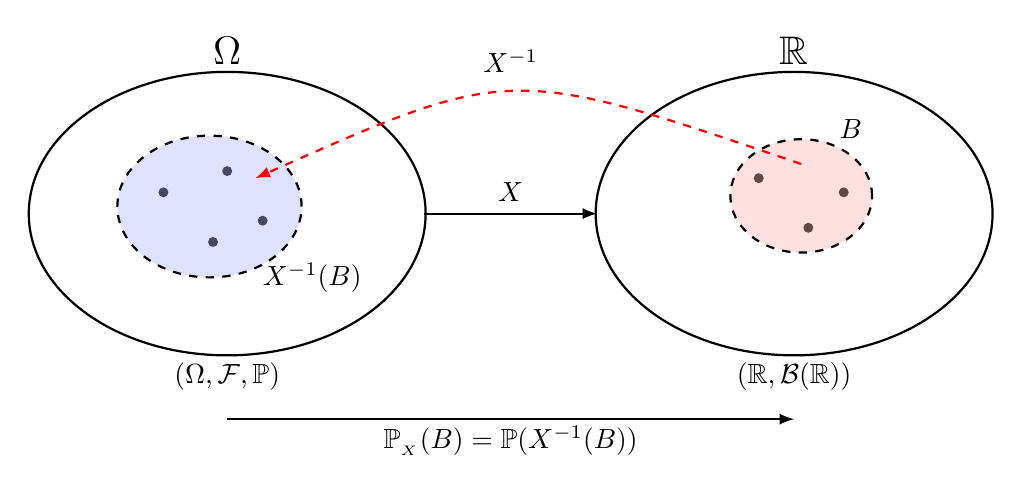
\begin{tikzpicture}[scale=0.9, >=latex]

% --- Sample space Omega ---
\draw[thick] (-4,0) ellipse (2.8 and 2.0);
\node at (-4,2.3) {\Large $\Omega$};
\node at (-4,-2.3) {$(\Omega,\mathcal F,\mathbb P)$};

% sample points in Omega 
\fill (-4.9,0.3) circle (2pt); % in X^{-1}(B)
\fill (-4,0.6) circle (2pt);
\fill (-4.2,-0.4) circle (2pt); % in X^{-1}(B)
\fill (-3.5,-0.1) circle (2pt);

% --- Subset in Omega: X^{-1}(B) ---
\draw[thick, dashed, fill=blue!30, fill opacity=0.4] (-4.25,0.1) ellipse (1.3 and 1.0);
\node at (-2.8,-0.9) {$X^{-1}(B)$};

% --- Real line / codomain ---
\draw[thick] (4,0) ellipse (2.8 and 2.0);
\node at (4,2.3) {\Large $\mathbb R$};
\node at (4,-2.3) {$(\mathbb R,\mathcal B(\mathbb R))$};

% image points in R 
\fill (3.5,0.5) circle (2pt); % in B
\fill (4.2,-0.2) circle (2pt);
\fill (4.7,0.3) circle (2pt); % in B

% --- Subset in R: B  ---
\draw[thick, dashed, fill=red!30, fill opacity=0.4] (4.1,0.25) ellipse (1.0 and 0.8);
\node at (4.8,1.2) {$B$};

% --- Arrow X (stays between the sets) ---
\draw[->, thick] (-1.22,0) -- (1.22,0);
\node at (0,0.3) {$X$};

% --- Dashed inverse image arrow ---
\draw[dashed, thick, red, ->] (4.1,0.7) .. controls (0,2.1) .. (-3.6,0.5);
\node at (0,2.15) {$X^{-1}$};

% --- Probability arrows ---
\draw[->, thick] (-4,-2.9) -- (4,-2.9);
\node at (0,-3.2) {$\mathbb P_{_X}(B)=\mathbb P(X^{-1}(B))$};

		\end{tikzpicture}
\caption{Probability Law For a Random Variable $X$.}
\label{fig:problaw}
	\end{center}
\end{figure}
\vskip 5mm

%%%%%%%%%%%%%%%%%%%%%%%%%%%%%%%%%%%%%%%%%%%%%%%%%%%%%%%%%%%%%%%%%%%%%%%%%%%%%%%%%%%%%%%%%%


A function called the distribution function of $X$ is one of the most important tools for working with random variables.
\vskip 5mm
\begin{defn}
Let $X$ be a random variable with a corresponding probability space $(\O,\F,\P)$. Then we define the {\bf\emph{distribution function}} $F_{_X}$ as
\[F_{_X}(x)=\P_{_X}\Big((-\infty,x]\Big)=\P\Big(\big\{\o\in\O:X(\o)\le x\big\}\Big).\]
\end{defn}

\ni {\bf\emph{Note}}: It can be shown that the distribution function $F_{X}$ completely determines the probability law $\P_{X}$; i.e., once we have defined the probability law for all sets $(-\infty,x]$, there is a unique way to extend this probability law to the Borel $\sigma$-algebra $\mathcal{B}(\R)$.\\

\ni There are a few distinguishing characteristics of a distribution which we list below.\\

\begin{thm}\label{thm:distribution}
Let $(\O,\F,\P)$ be a probability space and $X:\F\to\
R$ be a random variable with distribution function $F_{_X}$. Then the following properties hold.

	\begin{enumerate}
	
		\item $\ds\lim_{x\to-\infty}F_{_X}(x)=0$;
		\item $\ds\lim_{x\to\infty}F_{_X}(x)=1$;
		\item $F_{_X}$ is monotonically increasing everywhere; i.e., if $x\le y$, then $F_{_X}(x)\le F_{_X}(y)$.
		\item $F_{_X}$ is right-continuous; i.e., for all $x\in\R$ we have 
$\ds\lim_{\epsilon\to 0^+}F_{_X}(x+\epsilon)=F_{_X}(x)$. 
		
	\end{enumerate}
	
\end{thm}

\ni There are a limited number of types of random variables: discrete, continuous, singular, or a combination of the previous. In these notes we will only concern ourselves with the definitions of a discrete random variable.


%%%%%%%%%%%%%%%%%%%%%%%%%%%%%%%%%%%%%%%%%%%%%%%%%%%%%%%%%%%%%%%%%%%%%%%%%%%%%%%%%%%%%%%%%%%%%%%%%%%%%%
\section*{Discrete Random Variables:}
%%%%%%%%%%%%%%%%%%%%%%%%%%%%%%%%%%%%%%%%%%%%%%%%%%%%%%%%%%%%%%%%%%%%%%%%%%%%%%%%%%%%%%%%%%%%%%%%%%%%%%


\begin{defn}\label{def:discrete}
A random variable $X$ is called {\bf\emph{discrete}} if it takes at most countably many values $\{x_1, x_2, x_3, \dots\}$ and probabilities $p_i=\P(X = x_i)$ such that
\[\sum_{i} p_i = 1.\]
The function $p_{_X}:\mathbb{R} \to [0,1]$ defined by $p_{_X}(x)=\P(X = x)$
is called the \emph{probability mass function (pmf)} of $X$, and for any subset $A\subseteq\R$,
\[\P(X\in A)=\sum_{x_i\in A} p_{_X}(x_i).\]
\end{defn}

\begin{figure}[h!]
	\begin{center}
		\includegraphics[scale=0.6]{discrete_distribution_plot.jpeg}
\caption{Distribution Function for a Discrete Random Variable.}
\label{fig:drvdistribution}
	\end{center}
\end{figure}	

\ni Notice the step function behavior for a distribution function for discrete random variable. The right-continuity is clear from the graph.\\
	
%%%%%%%%%%%%%%%%%%%%%%%%%%%%%%%%%%%%%%%%%%%%%%%%%%%%%%
% Diagram of Discrete Prob Law
%%%%%%%%%%%%%%%%%%%%%%%%%%%%%%%%%%%%%%%%%%%%%%%%%%%%%%

\begin{figure}[h!]
	\begin{center}
		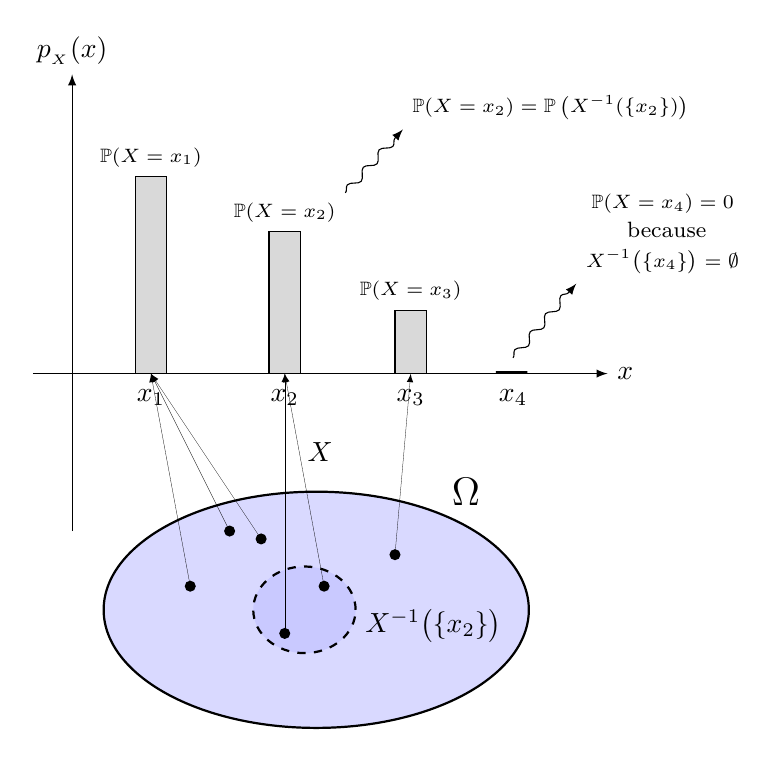
\begin{tikzpicture}[>=latex, scale=1.0]

% Axes
\draw[->] (-0.5,0) -- (6.8,0) node[right] {$x$};
\draw[->] (0,-2) -- (0,3.8) node[above] {$p_{_X}(x)$};

% x-values
\node at (1,-0.3) {$x_1$};
\node at (2.7,-0.3) {$x_2$};
\node at (4.3,-0.3) {$x_3$};
\node at (5.6,-0.3) (pointx4) {$x_4$};

% Histogram bars
\draw[fill=gray!30] (0.8,0) rectangle (1.2,2.5);
\draw[fill=gray!30] (2.5,0) rectangle (2.9,1.8);
\draw[fill=gray!30] (4.1,0) rectangle (4.5,0.8);
\draw[fill=gray!30, thick] (5.38,0.02) rectangle (5.78,0.02); % thin zero-height bar

% PMF labels above bars
\node[above, font=\scriptsize] at (1,2.5) {$\mathbb{P}(X=x_1)$};
\node[above, font=\scriptsize] at (2.7,1.8) (px2) {$\mathbb{P}(X=x_2)$};
\node[above, font=\scriptsize] at (4.3,0.8) {$\mathbb{P}(X=x_3)$};

%  Probability explanation label
\node[above right, font=\scriptsize] (exp2) at (4.2,3.1) 
    {$\mathbb{P}(X=x_2)=\mathbb{P}\left(X^{-1}(\{x_2\})\right)$};

% Squiggly arrow from PMF label to explanation label
\draw[->, thin, decorate, decoration={snake, amplitude=0.5mm, segment length=3mm}] 
    (px2.north east) -- (exp2.south west);

% Zero-probability explanation 
\node[below, font=\scriptsize] at (7.5,2.4) {$\mathbb{P}(X=x_4)=0$};
\node[font=\footnotesize] at (7.55,1.83) {because};
\node[below, font=\scriptsize] at (7.5,1.7) (px4) {$X^{-1}\big(\{x_4\}\big)=\emptyset$};

% Squiggly arrow from PMF to explanation label
\draw[->, thin, decorate, decoration={snake, amplitude=0.5mm, segment length=3mm}] 
    (5.6,0.2) -- (px4.south west);

% Omega set (draw FIRST)
\draw[thick, fill=blue!15] (3.1,-3.0) ellipse (2.7 and 1.5);
\node at (5,-1.5) {\Large $\Omega$};

% Subset X^{-1}(x2) (draw SECOND)
\draw[thick, dashed, fill=blue!30, fill opacity=0.4]
      (2.95,-3.0) ellipse (0.65 and 0.55);
\node[right] at (3.6,-3.2) {$X^{-1}\big(\{x_2\}\big)$};

% Sample points (draw LAST)
\fill (1.5,-2.7) circle (2pt);   % -> x1
\fill (2.4,-2.1) circle (2pt);   % -> x1
\fill (2,-2) circle (2pt);       % -> x1

\fill (2.7,-3.3) circle (2pt);   % -> x2
\fill (3.2,-2.7) circle (2pt);   % -> x2

\fill (4.1,-2.3) circle (2pt);   % -> x3

% Mapping arrows
\draw[->, ultra thin] (1.5,-2.7) -- (1,0);
\draw[->, ultra thin] (2.4,-2.1) -- (1,0);
\draw[->, ultra thin] (2,-2) -- (1,0);

\draw[->, ultra thin] (2.7,-3.3) -- (2.7,0);
\draw[->, ultra thin] (3.2,-2.7) -- (2.7,0);

\draw[->, ultra thin] (4.1,-2.3) -- (4.3,0);

% Label X
\node at (3.15,-1) {$X$};

		\end{tikzpicture}
\caption{Probability Law For a Discrete Random Variable.}
\label{fig:drvproblaw}	
	\end{center}
\end{figure}



%%%%%%%%%%%%%%%%%%%%%%%%%%%%%%%%%%%%%%%%%%%%%%%%%%%%%%%%%%%%%%%%%%%%%%%%%%%%%%%%%%%%%%%%%%%%%%%%%%%%%%
\section*{Theoretical Tools:}
%%%%%%%%%%%%%%%%%%%%%%%%%%%%%%%%%%%%%%%%%%%%%%%%%%%%%%%%%%%%%%%%%%%%%%%%%%%%%%%%%%%%%%%%%%%%%%%%%%%%%%

\noindent Once a discrete random variable is described by its probability mass function, we can compute numerical summaries that describe its typical behavior and variability.

\medskip

\begin{defn}
Let $X$ be a discrete random variable with pmf $p_{_X}(x)=\mathbb P(X=x)$.  

\begin{itemize}
\item The \textbf{expected value} (or mean) of $X$ is one measure of the ``center" of the probability distribution. It is computed as 
\[\mathbb{E}[X]=\sum_x x\,p_{_X}(x),\]
provided the sum converges absolutely. It is simply a weighted average.

\item The \textbf{variance} of $X$ is 
\[\mathrm{Var}(X)=\mathbb{E}\big[(X-\mathbb E[X])^2\big]=\sum_x (x-\mathbb{E}[X])^2 p_{_X}(x).\]
This numerical value is a measure of the average squared-distance from the mean which is the center mass of the probability distribution.The variance measures the spread of the distribution around its mean. A commonly used identity is
\[\mathrm{Var}(X)=\mathbb{E}[X^2]-(\mathbb{E}[X])^2.\]
\end{itemize}
\end{defn}

\medskip

\begin{thm*}[Linearity of Expectation]
If $X$ and $Y$ are discrete random variables and $a,b\in\mathbb{R}$, then
\[\mathbb{E}[aX+bY] = a\,\mathbb{E}[X]+b\,\mathbb{E}[Y].\]
This holds \emph{regardless of whether $X$ and $Y$ are independent}.
\end{thm*}

\vskip 2mm

\ni $\bullet$ This property makes expected value one of the most powerful tools in probability.

\vskip 5mm

\begin{thm*}
If $X$ and $Y$ are independent discrete random variables, then
\[\mathrm{Var}(X+Y)=\mathrm{Var}(X)+\mathrm{Var}(Y).\]
\end{thm*}

\medskip

\begin{thm*}[LOTUS]
If $g:\mathbb R\to\R$ is any function, then $Y=g(X)$ is also a discrete random variable with
\[\mathbb{E}[g(X)]=\sum_x g(x)\,p_{_X}(x).\]
\end{thm*}
This theorem is often referred to as the ``law of the unconscious statistician." Notice that to find the expected value of the random variable $g(X)$, we can use the mass function for $X$. Conveniently, we do not need to find the mass function for the new ranodm variable $g(X)$. This fact is frequently used to compute moments and transformations of random variables.


%%%%%%%%%%%%%%%%%%%%%%%%%%%%%%%%%%%%%%%%%%%%%%%%%%%%%%%%%%%%%%%%%%%%%%%%%%%%%%%%%%%%%%%%%%%%%%%%%%%%%%
\section*{Some Common Distributions:}
%%%%%%%%%%%%%%%%%%%%%%%%%%%%%%%%%%%%%%%%%%%%%%%%%%%%%%%%%%%%%%%%%%%%%%%%%%%%%%%%%%%%%%%%%%%%%%%%%%%%%%

Many discrete random variables that arise in applications fall into a small number of standard families.
Each distribution corresponds to a particular modeling situation. Understanding the assumptions behind
each model is often more important than memorizing formulas.

\medskip

%%%%%%%%%%%%%%%%%%%%%%%%%%%%%%%%%%%%%%%%%%%%%%%%%%%%%%%%%%%%%%%%%%%%%%%%%%%%
\subsection*{Bernoulli Distribution:}
%%%%%%%%%%%%%%%%%%%%%%%%%%%%%%%%%%%%%%%%%%%%%%%%%%%%%%%%%%%%%%%%%%%%%%%%%%%%
\vskip 2mm
A \emph{Bernoulli random variable} $X$ models a single experiment with two possible outcomes: 
\emph{success} or \emph{failure}.

\[X=\begin{cases}
1, & \text{with probability } p,\\
0, & \text{with probability } 1-p.
\end{cases}\]

The probability mass function is
\[\P(X=x)=p^x(1-p)^{1-x},\qquad x\in\{0,1\}.\]

\[\mathbb{E}[X]=p,\qquad\mathrm{Var}(X)=p(1-p).\]

\ni The Bernoulli distribution is the \emph{building block} for many other discrete distributions.

\medskip

%%%%%%%%%%%%%%%%%%%%%%%%%%%%%%%%%%%%%%%%%%%%%%%%%%%%%%%%%%%%%%%%%%%%%%%%%%%%
\subsection*{Binomial Distribution:}
%%%%%%%%%%%%%%%%%%%%%%%%%%%%%%%%%%%%%%%%%%%%%%%%%%%%%%%%%%%%%%%%%%%%%%%%%%%%
\vskip 2mm
Let $X$ be the number of successes in $n$ independent Bernoulli trials, each with success probability $p$.
Then $X$ has a \emph{Binomial distribution}, written $X\sim\mathrm{Binomial}(n,p)$.

\[\P(X=k)=\binom{n}{k}p^k(1-p)^{n-k},\qquad k=0,1,\dots,n.\]

\[\mathbb{E}[X]=np,\qquad\mathrm{Var}(X)=np(1-p).\]

\medskip

\ni \emph{Connection to Bernoulli:} If $X_1,\dots,X_n$ are independent Bernoulli$(p)$ random variables, then
\[X=X_1+\cdots+X_n\sim\mathrm{Binomial}(n,p).\]

\ni Thus, the binomial distribution counts the total number of successes across repeated Bernoulli trials.

\medskip

%%%%%%%%%%%%%%%%%%%%%%%%%%%%%%%%%%%%%%%%%%%%%%%%%%%%%%%%%%%%%%%%%%%%%%%%%%%%
\subsection*{Geometric Distribution:}
%%%%%%%%%%%%%%%%%%%%%%%%%%%%%%%%%%%%%%%%%%%%%%%%%%%%%%%%%%%%%%%%%%%%%%%%%%%%
\vskip 2mm
A \emph{Geometric random variable} $X$ counts the number of independent Bernoulli$(p)$ trials needed to obtain
the \emph{first} success.

\[\P(X=k)=(1-p)^{k-1}p,\qquad k=1,2,3,\dots\]

\[\mathbb{E}[X]=\frac{1}{p},\qquad\mathrm{Var}(X)=\frac{1-p}{p^2}.\]

\medskip

\ni \emph{Memoryless property:} For all $m,n\ge 1$,
\[\P(X>m+n\mid X>m)=\P(X>n).\]

\ni This property is unique among discrete distributions and makes the geometric distribution
particularly useful for modeling waiting times.

\medskip

%%%%%%%%%%%%%%%%%%%%%%%%%%%%%%%%%%%%%%%%%%%%%%%%%%%%%%%%%%%%%%%%%%%%%%%%%%%%
\subsection*{Negative Binomial Distribution:}
%%%%%%%%%%%%%%%%%%%%%%%%%%%%%%%%%%%%%%%%%%%%%%%%%%%%%%%%%%%%%%%%%%%%%%%%%%%%
\vskip 2mm
A \emph{Negative Binomial random variable} $X$ generalizes the geometric distribution.
It counts the number of trials required to obtain $r$ successes.

\[\P(X=k)=\binom{k-1}{r-1}p^r(1-p)^{k-r},\qquad k=r,r+1,\dots\]

\[\mathbb{E}[X]=\frac{r}{p},\qquad \mathrm{Var}(X)=\frac{r(1-p)}{p^2}.\]

\ni When $r=1$, the negative binomial distribution reduces to the geometric distribution.

\medskip

%%%%%%%%%%%%%%%%%%%%%%%%%%%%%%%%%%%%%%%%%%%%%%%%%%%%%%%%%%%%%%%%%%%%%%%%%%%%
\subsection*{Hypergeometric Distribution:}
%%%%%%%%%%%%%%%%%%%%%%%%%%%%%%%%%%%%%%%%%%%%%%%%%%%%%%%%%%%%%%%%%%%%%%%%%%%%
\vskip 2mm
A \emph{Hypergeometric random variable} $X$ models sampling \emph{without replacement}
from a finite population.
\vskip 5mm
Suppose a population of size $N$ contains $K$ successes and $N-K$ failures.
If $n$ items are selected without replacement and $X$ is the number of successes, then

\[\P(X=k)=\frac{\binom{K}{k}\binom{N-K}{n-k}}{\binom{N}{n}},\qquad k=0,1,\dots,n.\]

\[\mathbb{E}[X]=\frac{nK}{N}.\]

\medskip

\ni \textbf{Comparison with the Binomial distribution.}

\begin{itemize}
\item Binomial: sampling \emph{with} replacement (or independent trials)
\item Hypergeometric: sampling \emph{without} replacement
\end{itemize}

\ni When the population size $N$ is large relative to $n$, the hypergeometric distribution
is well approximated by a binomial distribution with $p=K/N$.

\medskip

%%%%%%%%%%%%%%%%%%%%%%%%%%%%%%%%%%%%%%%%%%%%%%%%%%%%%%%%%%%%%%%%%%%%%%%%%%%%
\subsection*{Poisson Distribution:}
%%%%%%%%%%%%%%%%%%%%%%%%%%%%%%%%%%%%%%%%%%%%%%%%%%%%%%%%%%%%%%%%%%%%%%%%%%%%
\vskip 2mm
A \emph{Poisson random variable} $X$ with rate parameter $\lambda>0$ has pmf
\[\P(X=k)=\frac{\lambda^k e^{-\lambda}}{k!}, \qquad k=0,1,2,\dots\]

\[\mathbb{E}[X]=\lambda,\qquad \mathrm{Var}(X)=\lambda.\]

\medskip

\ni The Poisson distribution is commonly used to model the number of events
occurring in a fixed interval of time or space when events occur independently
at a constant average rate.


%%%%%%%%%%%%%%%%%%%%%%%%%%%%%%%%%%%%%%%%%%%%%%%%%%%%%%%%%%%%%%%%%%%%%%%%%%%%
\subsection*{Poisson Distribution as a Limit of the Binomial:}
%%%%%%%%%%%%%%%%%%%%%%%%%%%%%%%%%%%%%%%%%%%%%%%%%%%%%%%%%%%%%%%%%%%%%%%%%%%%
\vskip 2mm
The Poisson distribution can be derived as a limiting case of the binomial distribution
when the number of trials is large and the probability of success is small. Let $X_n \sim \mathrm{Binomial}(n,p_n)$, where $p_n$ depends on $n$ in such a way that
\[np_n \to \lambda > 0 \quad \text{as } n\to\infty.\]
Equivalently, we take $p_n=\lambda/n$ and compute the limiting value of the probability that $X_n=k$ for a fixed nonnegative integer $k$:

\small
\beq
\ds\lim_{n\to\infty}\P(X_n=k)&=&\ds\lim_{n\to\infty}\underbrace{\binom{n}{k}}_{\text{Expand}}\left(\frac{\lambda}{n}\right)^k\underbrace{\left(1-\frac{\lambda}{n}\right)^{n-k}}_{\substack{\text{Break into two}\\\text{terms}}}\\
\\
&=&\ds\lim_{n\to\infty}\overbrace{\frac{n(n-1)\cdots(n-k+1)}{k!}}^{\text{Factor $n$ from each term}}\cdot\frac{\lambda^k}{n^k}\cdot\left(1-\frac{\lambda}{n}\right)^n
\left(1-\frac{\lambda}{n}\right)^{-k}\\
\\
&=&\ds\lim_{n\to\infty}\ds\frac{\cancel{n^k}}{k!}\cdot\left(1-\frac{1}{n}\right)\left(1-\frac{2}{n}\right)\cdots
\left(1-\frac{k-1}{n}\right)\cdot\frac{\lambda^k}{\cancel{n^k}}\cdot\left(1-\frac{\lambda}{n}\right)^n
\left(1-\frac{\lambda}{n}\right)^{-k}\\
\\
&=&\ds\lim_{n\to\infty}\frac{\lambda^k}{k!}\cdot\cancelto{1}{\left(1-\frac{1}{n}\right)}\cdots\cancelto{1}{\left(1-\frac{k-1}{n}\right)}\cdot\cancelto{\,e^{-\lambda}}{\left(1-\frac{\lambda}{n}\right)^n}
\;\;\cancelto{1}{\left(1-\frac{\lambda}{n}\right)^{-k}}\\
\\
&=&\ds\frac{e^{-\lambda}\lambda^k}{k!}
\eeq

\normalsize

After putting everything together we see
\[\P(X_n=k)\;\overset{n}{\longrightarrow}\;\frac{e^{-\lambda}\lambda^k}{k!},\qquad k=0,1,2,\dots\]
This is the mass function of a Poisson random variable with rate parameter $\lambda=np_n$. This result explains why the Poisson distribution is an appropriate model for rare events occurring in a large number of trials, such as defects in manufacturing, phone calls arriving at a call center, or radioactive decay events.


\medskip

%%%%%%%%%%%%%%%%%%%%%%%%%%%%%%%%%%%%%%%%%%%%%%%%%%%%%%%%%%%%%%%%%%%%%%%%%%%%
\paragraph*{Summary of Connections:}
%%%%%%%%%%%%%%%%%%%%%%%%%%%%%%%%%%%%%%%%%%%%%%%%%%%%%%%%%%%%%%%%%%%%%%%%%%%%

\begin{itemize}
\item Bernoulli: one trial, success or failure
\item Binomial: number of successes in many Bernoulli trials
\item Geometric: waiting time for first success
\item Negative Binomial: waiting time for $r$ successes
\item Hypergeometric: successes without replacement
\item Poisson: rare events over time or space
\end{itemize}

\vskip 1cm
\hrule
\vskip 1cm

%%%%%%%%%%%%%%%%%%%%%%%%%%%%%%%%%%%%%%%%%%%%%%%%%%%%%%%%%%%%%%%%%%%%%%%%%%%%%%%%%%%%%%%%%%%%%%%%%%%%%%
\section*{Foundational Examples: Inverse Images and Probabilities}
%%%%%%%%%%%%%%%%%%%%%%%%%%%%%%%%%%%%%%%%%%%%%%%%%%%%%%%%%%%%%%%%%%%%%%%%%%%%%%%%%%%%%%%%%%%%%%%%%%%%%%

The key idea behind discrete random variables is that probabilities of numerical events
are computed by pulling them back to the underlying sample space.
The following examples emphasize the identity
\[
\mathbb P(X\in A)=\mathbb P\big(X^{-1}(A)\big).
\]

\medskip

%%%%%%%%%%%%%%%%%%%%%%%%%%%%%%%%%%%%%%%%%%%%%%%%%%%%%%%%%%%%%%%%%%%%%%%%%%%%
\textbf{Example 1: Partitioning the Unit Interval}
%%%%%%%%%%%%%%%%%%%%%%%%%%%%%%%%%%%%%%%%%%%%%%%%%%%%%%%%%%%%%%%%%%%%%%%%%%%%
\vskip 2mm
Choose a number $\omega$ uniformly at random from the interval $(0,1)$.
Define a random variable $X$ by
\[
X(\omega)=
\begin{cases}
0, & 0<\omega<\frac{1}{3},\\[4pt]
1, & \frac{1}{3}\le \omega<1.
\end{cases}
\]

\medskip

\ni The sample space is $\Omega=(0,1)$ equipped with the uniform probability measure.
The random variable $X$ takes only the values $\{0,1\}$.

\medskip

\begin{itemize}
\item $X^{-1}(\{0\})=(0,\tfrac13)$
\item $X^{-1}(\{1\})=[\tfrac13,1)$
\end{itemize}

\medskip

Thus,
\[
\mathbb P(X=0)=\mathbb P\big((0,\tfrac13)\big)=\ds\frac{1}{3},
\qquad
\mathbb P(X=1)=\mathbb P\big([\tfrac13,1)\big)=\ds\frac{2}{3}.
\]

\medskip

For example, if $A=\{1\}$, then
\[\P(X\in A)=\P(X=1)=\P\big(X^{-1}(\{1\})\big)=\P\big([\tfrac13,1)\big)=\ds\frac{2}{3}.\]

\vskip 1cm

%%%%%%%%%%%%%%%%%%%%%%%%%%%%%%%%%%%%%%%%%%%%%%%%%%%%%%%%%%%%%%%%%%%%%%%%%%%%
\textbf{Example 2: Coarsening Outcomes of a Die Roll}
%%%%%%%%%%%%%%%%%%%%%%%%%%%%%%%%%%%%%%%%%%%%%%%%%%%%%%%%%%%%%%%%%%%%%%%%%%%%
\vskip 2mm
Roll a fair six-sided die once. Let $\Omega=\{1,2,3,4,5,6\}$ with
$\P(\{\omega\})=1/6$ for each outcome. Define a random variable $X$ by
\[X(\omega)=\begin{cases}
-1, & \omega\in\{1,2\},\\
0, & \omega\in\{3,4\},\\
1, & \omega\in\{5,6\}.
\end{cases}\]

\medskip

\ni The random variable $X$ groups together outcomes of the die into three numerical categories.

\medskip

\begin{itemize}
\item $X^{-1}(\{-1\})=\{1,2\}$
\item $X^{-1}(\{0\})=\{3,4\}$
\item $X^{-1}(\{1\})=\{5,6\}$
\end{itemize}

\medskip

Therefore,
\[\P(X=-1)=\frac{2}{6},\quad\P(X=0)=\frac{2}{6},\quad\P(X=1)=\frac{2}{6}.\]

\medskip

For the set $A=\{-1,1\}$,
\[X^{-1}(A)=\{1,2,5,6\},\qquad\P(X\in A)=\frac{4}{6}.\]

\vfill\eject

%%%%%%%%%%%%%%%%%%%%%%%%%%%%%%%%%%%%%%%%%%%%%%%%%%%%%%%%%%%%%%%%%%%%%%%%%%
\textbf{Example 3: A Threshold Event}
%%%%%%%%%%%%%%%%%%%%%%%%%%%%%%%%%%%%%%%%%%%%%%%%%%%%%%%%%%%%%%%%%%%%%%%%%%%%
\vskip 2mm
Choose $\omega$ uniformly at random from $(0,1)$ and define
\[X(\omega)=\begin{cases}
0, & 0<\omega<0.8,\\
1, & 0.8\le \omega<1.
\end{cases}\]

\medskip

\ni Let $A=\{1\}$. Then
\[X^{-1}(A)=[0.8,1).\]

\medskip

Therefore,
\[\P(X\in A)=\P(X=1)=\P\big([0.8,1)\big)=0.2.\]

\medskip

This example illustrates that probabilities are not assigned directly to numbers,
but to subsets of the sample space determined by the random variable.

\vskip 1cm

%%%%%%%%%%%%%%%%%%%%%%%%%%%%%%%%%%%%%%%%%%%%%%%%%%%%%%%%%%%%%%%%%%%%%%%%%%%%
\textbf{Example 4 (From outcomes to values)}  
%%%%%%%%%%%%%%%%%%%%%%%%%%%%%%%%%%%%%%%%%%%%%%%%%%%%%%%%%%%%%%%%%%%%%%%%%%%%
\vskip 2mm
Let $\Omega=(0,1)$ with probability measure given by uniform length, so that
$\P((a,b))=b-a$ for $0<a<b<1$.

Define a random variable $X:\Omega\to\{0,1\}$ by
\[X(\omega)=\begin{cases}
0, & 0<\omega<\frac{1}{3},\\[4pt]
1, & \frac{1}{3}\le \omega<1.
\end{cases}\]

\begin{enumerate}
\item Find $\P(X=0)$ and $\P(X=1)$.
\item Find $\P(X\in\{0,1\})$.
\end{enumerate}

\begin{solutionbox}
We compute probabilities by identifying preimages in $\Omega$.

\[X^{-1}(\{0\})=(0,\ds\frac{1}{3}),\qquad X^{-1}(\{1\})=[\ds\frac{1}{3},1).\]

Thus,
\[\P(X=0)=\P\big((0,\tfrac{1}{3})\big)=\tfrac{1}{3},\qquad\P(X=1)=\P\big([\tfrac{1}{3},1)\big)=\ds\frac{2}{3}.\]

Since $X$ only takes the values $0$ and $1$,
\[X^{-1}(\{0,1\})=(0,1),\]
and therefore
\[\P(X\in\{0,1\})=\P((0,1))=1.\]
\end{solutionbox}

\vfill\eject

%%%%%%%%%%%%%%%%%%%%%%%%%%%%%%%%%%%%%%%%%%%%%%%%%%%%%%%%%%%%%%%%%%%%%%%%%%%%
\textbf{Example 5 (Event mapping)}  
%%%%%%%%%%%%%%%%%%%%%%%%%%%%%%%%%%%%%%%%%%%%%%%%%%%%%%%%%%%%%%%%%%%%%%%%%%%%
\vskip 5mm
Let $\Omega=(0,1)$ and define
\[X(\omega)=\begin{cases}
-1, & 0<\omega<\tfrac{1}{4},\\
0, & \tfrac{1}{4}\le \omega<\tfrac{3}{4},\\
2, & \tfrac{3}{4}\le \omega<1.
\end{cases}\]

\begin{enumerate}
\item Find $\P(X\le 0)$.
\item Find $\P(X\in\{-1,2\})$.
\end{enumerate}

\begin{solutionbox}
\[X^{-1}((-\infty,0])=(0,\tfrac{3}{4}),\]
since $X(\omega)\le 0$ when $\omega<\tfrac{3}{4}$. Thus,
\[\P(X\le 0)=\P\big((0,\tfrac{3}{4})\big)=\ds\frac{3}{4}.\]

For the second event,
\[X^{-1}(\{-1,2\})=(0,\ds\frac{1}{4})\cup[\ds\frac{3}{4},1).\]

Therefore,
\[\P(X\in\{-1,2\})=\ds\frac{1}{4}+\ds\frac{1}{4}=\ds\frac{1}{2}.\]
\end{solutionbox}

\medskip

%%%%%%%%%%%%%%%%%%%%%%%%%%%%%%%%%%%%%%%%%%%%%%%%%%%%%%%%%%%%%%%%%%%%%%%%%%%%
\textbf{Example 6 (Distribution function via preimages)}
%%%%%%%%%%%%%%%%%%%%%%%%%%%%%%%%%%%%%%%%%%%%%%%%%%%%%%%%%%%%%%%%%%%%%%%%%%%%
\vskip 2mm  
Let $\Omega=(0,1)$ and define
\[X(\omega)=\begin{cases}
1, & 0<\omega<\tfrac{1}{2},\\
3, & \tfrac{1}{2}\le \omega<1.
\end{cases}\]

\begin{enumerate}
\item Find the distribution function $F_{_X}(x)=\mathbb P(X\le x)$.
\item Sketch $F_{_X}(x)$.
\end{enumerate}

\begin{solutionbox}
We compute $F_{_X}(x)$ by identifying $X^{-1}((-\infty,x])$.

\begin{itemize}
\item If $x<1$, then $X^{-1}((-\infty,x])=\emptyset$, so $F_{_X}(x)=0$.
\item If $1\le x<3$, then $X^{-1}((-\infty,x])=(0,\ds\frac{1}{2})$, so
\[F_{_X}(x)=\ds\frac{1}{2}.\]
\item If $x\ge 3$, then $X^{-1}((-\infty,x])=(0,1)$, so $F_{_X}(x)=1$.
\end{itemize}

Thus,
\[F_{_X}(x)=\begin{cases}
0, & x<1,\\
\tfrac{1}{2}, & 1\le x<3,\\
1, & x\ge 3.
\end{cases}\]

This illustrates the step-function behavior of the distribution function for a discrete random variable.
\end{solutionbox}

\vskip 1cm
\hrule
\vskip 1cm

%%%%%%%%%%%%%%%%%%%%%%%%%%%%%%%%%%%%%%%%%%%%%%%%%%%%%%%%%%%%%%%%%%%%%%%%%%%%%%%%%%%%%%%%%%%%%%%%%%%%%%
\section*{Conceptual Quiz: Preimages of Random Variables}
%%%%%%%%%%%%%%%%%%%%%%%%%%%%%%%%%%%%%%%%%%%%%%%%%%%%%%%%%%%%%%%%%%%%%%%%%%%%%%%%%%%%%%%%%%%%%%%%%%%%%%

The purpose of this quiz is to reinforce the idea that probabilities involving a random variable
are computed using inverse images:
\[
\mathbb P(X\in A)=\mathbb P\big(X^{-1}(A)\big).
\]

\medskip

\textbf{Question:} Let $\Omega=(0,1)$ with the uniform probability measure.
Define a random variable $X:\Omega\to\mathbb R$ by
\[
X(\omega)=
\begin{cases}
-1, & 0<\omega<0.2,\\[4pt]
0,  & 0.2\le \omega<0.7,\\[4pt]
1,  & 0.7\le \omega<1.
\end{cases}
\]

Let $A=\{-1,1\}$.

\medskip

\begin{enumerate}
\item[(a)] Which of the following sets is \emph{exactly} $X^{-1}(A)$?

\[
\begin{array}{ll}
\text{(i)} & (0,0.2)\cup(0.7,1) \\[4pt]
\text{(ii)} & \{-1,1\} \\[4pt]
\text{(iii)} & (0,1)\setminus[0.2,0.7) \\[4pt]
\text{(iv)} & (0.2,0.7)
\end{array}
\]

\item[(b)] In one or two sentences, explain \emph{why} your choice in part (a) is correct.

\item[(c)] Without performing any calculations, explain how you would compute
\[
\mathbb P(X\in A).
\]

\item[(d)] What is the set $X(A)$? Is this set useful for computing probabilities?
Briefly explain.
\end{enumerate}

\medskip

\begin{solutionbox}
\begin{enumerate}
\item[(a)] The correct answer is \textbf{(i)}:
\[
X^{-1}(\{-1,1\})=(0,0.2)\cup(0.7,1).
\]

\item[(b)] The inverse image consists of all outcomes $\omega\in\Omega$ whose
assigned value under $X$ lies in the set $\{-1,1\}$.

\item[(c)] We compute
\[
\mathbb P(X\in A)=\mathbb P\big(X^{-1}(A)\big)
\]
by finding the probability (length) of the subset
$(0,0.2)\cup(0.7,1)\subset(0,1)$.

\item[(d)] The image of the set $A$ is
\[
X(A)=\{X(-1),X(1)\}.
\]
However, $-1$ and $1$ are not elements of the sample space $\Omega=(0,1)$,
so $X(A)$ is not meaningful in this context.

Even when $A\subset\Omega$, the set $X(A)$ lives in $\mathbb R$ and does not correspond
to an event in the sample space. Probabilities are always assigned to subsets of $\Omega$,
which is why inverse images are essential.
\end{enumerate}
\end{solutionbox}


\vskip 1cm
\hrule
\vskip 1cm\

%%%%%%%%%%%%%%%%%%%%%%%%%%%%%%%%%%%%%%%%%%%%%%%%%%%%%%%%%%%%%%%%%%%%%%%%%%%%%%%%%%%%%%%%%%%%%%%%%%%%%%
\section*{Paired Example: Preimages in a Finite Sample Space}
%%%%%%%%%%%%%%%%%%%%%%%%%%%%%%%%%%%%%%%%%%%%%%%%%%%%%%%%%%%%%%%%%%%%%%%%%%%%%%%%%%%%%%%%%%%%%%%%%%%%%%

This example mirrors the previous quiz, but uses a finite sample space to emphasize that
the same ideas apply regardless of whether $\Omega$ is continuous or discrete.

\medskip

\textbf{Question:} Roll a fair six-sided die once.
Let $\Omega=\{1,2,3,4,5,6\}$ with $\mathbb P(\{\omega\})=1/6$ for each outcome.
Define a random variable $X:\Omega\to\mathbb R$ by
\[
X(\omega)=
\begin{cases}
-1, & \omega\in\{1,2\},\\
0,  & \omega\in\{3,4\},\\
1,  & \omega\in\{5,6\}.
\end{cases}
\]

Let $A=\{-1,1\}$.

\medskip

\begin{enumerate}
\item[(a)] Find the set $X^{-1}(A)$.

\item[(b)] Compute $\mathbb P(X\in A)$.

\item[(c)] What is the set $X(A)$?

\item[(d)] Explain why $X(A)$ is not useful for computing probabilities.
\end{enumerate}

\medskip

\begin{solutionbox}
\begin{enumerate}
\item[(a)] 
\[
X^{-1}(\{-1,1\})=\{1,2,5,6\}.
\]

\item[(b)] 
\[
\mathbb P(X\in A)=\mathbb P(\{1,2,5,6\})=\frac{4}{6}.
\]

\item[(c)] 
\[
X(A)=\{X(-1),X(1)\}.
\]
Since $-1$ and $1$ are not elements of $\Omega$, this expression is not meaningful.

\item[(d)] 
Probabilities are assigned to subsets of the sample space $\Omega$.
The set $X(A)$ lies in $\mathbb R$ and does not correspond to an event,
so it cannot be assigned a probability.
\end{enumerate}
\end{solutionbox}


\vskip 1cm
\hrule
\vskip 1cm


%%%%%%%%%%%%%%%%%%%%%%%%%%%%%%%%%%%%%%%%%%%%%%%%%%%%%%%%%%%%%%%%%%%%%%%%%%%%%%%%%%%%%%%%%%%%%%%%%%%%%%
\section*{Reflection: Why Inverse Images Matter}
%%%%%%%%%%%%%%%%%%%%%%%%%%%%%%%%%%%%%%%%%%%%%%%%%%%%%%%%%%%%%%%%%%%%%%%%%%%%%%%%%%%%%%%%%%%%%%%%%%%%%%

In the previous examples, probabilities involving the random variable $X$
were always computed using inverse images.

\medskip

\textbf{Reflection Prompt.}

In your own words, respond to the following:

\begin{itemize}
\item Why do we compute probabilities using $X^{-1}(A)$ rather than $X(A)$?
\item Where does probability \emph{actually live}: on the values of $X$ or on the sample space $\Omega$?
\item Describe one mistake a student might make if they confuse $X^{-1}(A)$ with $X(A)$.
\end{itemize}

\medskip

\ni Your response should focus on ideas and explanations rather than calculations.


%\vskip 1cm
%\hrule
%\vskip 1cm
%
%
%%%%%%%%%%%%%%%%%%%%%%%%%%%%%%%%%%%%%%%%%%%%%%%%%%%%%%%%%%%%%%%%%%%%%%%%%%%%%%%%%%%%%%%%%%%%%%%%%%%%%%%
%\section*{Multiple-Choice Question: Common Misconceptions About Preimages}
%%%%%%%%%%%%%%%%%%%%%%%%%%%%%%%%%%%%%%%%%%%%%%%%%%%%%%%%%%%%%%%%%%%%%%%%%%%%%%%%%%%%%%%%%%%%%%%%%%%%%%%
%
%\textbf{Question.}
%
%Roll a fair six-sided die once.
%Let $\Omega=\{1,2,3,4,5,6\}$ with $\mathbb P(\{\omega\})=1/6$ for each outcome.
%Define a random variable $X:\Omega\to\mathbb R$ by
%\[
%X(\omega)=
%\begin{cases}
%-1, & \omega\in\{1,2\},\\
%0,  & \omega\in\{3,4\},\\
%1,  & \omega\in\{5,6\}.
%\end{cases}
%\]
%
%Let $A=\{-1,1\}$.
%
%\medskip
%
%Which of the following correctly represents the event whose probability is
%$\mathbb P(X\in A)$?
%
%\medskip
%
%\begin{enumerate}
%\item[(A)] $\{-1,1\}$
%
%\item[(B)] $X(A)$
%
%\item[(C)] $X^{-1}(A)$
%
%\item[(D)] $\{1,2,5,6\}$
%
%\item[(E)] $\{-1,0,1\}$
%\end{enumerate}
%
%\medskip
%
%\textbf{Correct Answer:} \textbf{(D)}
%
%\medskip
%
%\begin{solutionbox}
%We are asked to identify the \emph{event} whose probability equals $\mathbb P(X\in A)$.
%
%By definition,
%\[
%\mathbb P(X\in A)=\mathbb P\big(X^{-1}(A)\big).
%\]
%Here,
%\[
%X^{-1}(\{-1,1\})=\{1,2,5,6\}.
%\]
%Thus the correct answer is \textbf{(D)}.
%\end{solutionbox}
%
%----------------------------------------------------------------------------------
% INSTRUCTOR NOTES (COMMENTED OUT)
%
% Purpose:
% This question is designed to diagnose common misconceptions about inverse images
% and the meaning of probabilities involving random variables.
%
% Distractor diagnostics:
%
% (A) {-1,1}
%   - Confuses values of the random variable with events.
%   - Student attempts to assign probability directly in R instead of Omega.
%
% (B) X(A)
%   - Confuses image with inverse image.
%   - Indicates symbol manipulation without conceptual grounding.
%
% (C) X^{-1}(A)
%   - Conceptually correct but incomplete.
%   - Student understands inverse images but has not evaluated them as subsets of Omega.
%
% (D) {1,2,5,6}
%   - Correct.
%   - Explicitly identifies the event in the sample space.
%
% (E) {-1,0,1}
%   - Treats the range of X as the event.
%   - Suggests confusion between the distribution of X and the sample space.
%
% Suggested follow-up question:
% "Why is option (C) conceptually correct but not the best answer?"
% Expected answer: Probabilities require explicit subsets of Omega, not formal expressions.
%----------------------------------------------------------------------------------


\vskip 1cm
\hrule
\vskip 1cm

%%%%%%%%%%%%%%%%%%%%%%%%%%%%%%%%%%%%%%%%%%%%%%%%%%%%%%%%%%%%%%%%%%%%%%%%%%%%%%%%%%%%%%%%%%%%%%%%%%%%%%
\section*{Additional Practice Problems: Common Distributions}
%%%%%%%%%%%%%%%%%%%%%%%%%%%%%%%%%%%%%%%%%%%%%%%%%%%%%%%%%%%%%%%%%%%%%%%%%%%%%%%%%%%%%%%%%%%%%%%%%%%%%%

\textbf{Problem 1 (Bernoulli).}  
A machine produces items that are defective with probability $0.02$. Let $X$ be a Bernoulli random variable
that equals $1$ if a randomly selected item is defective and $0$ otherwise. Write down the pmf, the expected value, and the variance.


\begin{solutionbox}
$X\sim\mathrm{Bernoulli}(0.02)$.

\[\mathbb{E}[X]=0.02,\qquad \mathrm{Var}(X)=0.02(0.98)=0.0196.\]
\end{solutionbox}

\medskip

\textbf{Problem 2 (Binomial).}  
A fair coin is tossed $20$ times. Let $X$ be the number of heads.

\begin{enumerate}
\item Identify the distribution of $X$.
\item Compute $\P(X=12)$.
\item Find $\mathbb{E}[X]$ and $\mathrm{Var}(X)$.
\end{enumerate}

\begin{solutionbox}
$X\sim\mathrm{Binomial}(20,0.5)$.

\[\P(X=12)=\binom{20}{12}(0.5)^{20}.\]

\[\mathbb{E}[X]=20(0.5)=10, \qquad \mathrm{Var}(X)=20(0.5)(0.5)=5.\]
\end{solutionbox}

\medskip

\textbf{Problem 3 (Geometric).}  
Each attempt to connect to a wireless network succeeds with probability $0.3$.
Let $X$ be the number of attempts until the first successful connection.

\begin{enumerate}
\item Find $\mathbb P(X=4)$.
\item Find $\mathbb P(X>4)$.
\item Compute $\mathbb E[X]$.
\end{enumerate}

\begin{solutionbox}
$X\sim\mathrm{Geometric}(0.3)$.

\[\P(X=4)=(0.7)^3(0.3).\]

\[\P(X>4)=(0.7)^4.\]

\[\mathbb{E}[X]=\frac{1}{0.3}\approx 3.33.\]
\end{solutionbox}

\medskip

\textbf{Problem 4 (Negative Binomial).}  
A basketball player makes each free throw with probability $0.8$.
Let $X$ be the number of shots required for the player to make $3$ free throws.

\begin{enumerate}
\item Identify the distribution of $X$.
\item Find $\mathbb{E}[X]$.
\end{enumerate}

\begin{solutionbox}
$X\sim\mathrm{NegativeBinomial}(r=3,p=0.8)$.

\[\mathbb{E}[X]=\frac{3}{0.8}=3.75.\]
\end{solutionbox}

\medskip

\textbf{Problem 5 (Hypergeometric).}  
An urn contains $8$ red balls and $12$ blue balls. Five balls are drawn at random without replacement.
Let $X$ be the number of red balls selected.

\begin{enumerate}
\item Identify the distribution of $X$.
\item Compute $\P(X=2)$.
\item Find $\mathbb{E}[X]$.
\end{enumerate}

\begin{solutionbox}
$X\sim\mathrm{Hypergeometric}(N=20,K=8,n=5)$.

\[\P(X=2)=\frac{\binom{8}{2}\binom{12}{3}}{\binom{20}{5}}.\]

\[\mathbb{E}[X]=5\cdot\frac{8}{20}=2.\]
\end{solutionbox}

\medskip

\textbf{Problem 6 (Binomial vs. Hypergeometric).}  
A shipment contains $1000$ items, $30$ of which are defective. A quality inspector selects $10$ items.

\begin{enumerate}
\item Which distribution exactly models the number of defective items selected?
\item Which distribution provides a reasonable approximation?
\end{enumerate}

\begin{solutionbox}
\begin{itemize}
\item The exact distribution is Hypergeometric$(N=1000,K=30,n=10)$.
\item Since the population is large relative to the sample size, a Binomial$(n=10,p=0.03)$
provides a good approximation.
\end{itemize}
\end{solutionbox}

\medskip

\textbf{Problem 7 (Poisson).}  
Calls arrive at a call center at an average rate of $4$ per hour.
Let $X$ be the number of calls in one hour.

\begin{enumerate}
\item Identify the distribution of $X$.
\item Compute $\P(X=0)$.
\item Compute $\P(X\ge 2)$.
\end{enumerate}

\begin{solutionbox}
$X\sim\mathrm{Poisson}(4)$.

\[\P(X=0)=e^{-4}.\]

\[\P(X\ge 2)=1-\P(X=0)-\P(X=1)=1-e^{-4}(1+4).\]
\end{solutionbox}

\medskip

\textbf{Problem 8 (Poisson Approximation to the Binomial).}  
A factory produces $10{,}000$ light bulbs, each of which has probability $0.0005$ of being defective.
Let $X$ be the number of defective bulbs.

\begin{enumerate}
\item Identify the exact distribution of $X$.
\item Identify an appropriate approximation.
\item State the parameter of the approximating distribution.
\end{enumerate}

\begin{solutionbox}
\begin{itemize}
\item $X\sim\mathrm{Binomial}(10{,}000,0.0005)$.
\item A Poisson approximation is appropriate since $n$ is large and $p$ is small.
\item $\lambda = np = 5$, so $X\approx\mathrm{Poisson}(5)$.
\end{itemize}
\end{solutionbox}


%%%%%%%%%%%%%%%%%%%%%%%%%%%%%%%%%%%%%%%%%%%%%%%%%%%%%%%%%%%%%%%%%%%%%%%%%%%%%%%%%%%%%%%%%%%%%%%%%%%%%%%
%\section*{The R Code:} 
%%%%%%%%%%%%%%%%%%%%%%%%%%%%%%%%%%%%%%%%%%%%%%%%%%%%%%%%%%%%%%%%%%%%%%%%%%%%%%%%%%%%%%%%%%%%%%%%%%%%%%%
% Here is the R code used for the above simulations.
%\vspace*{2mm}
%\small 
%\begin{lstlisting}[language=R]
%
%
%
%\end{lstlisting}


\vskip 1cm
\hrule
\vskip 5mm
\begin{center}
\bf Please let me know if you have any questions, comments, or corrections!
\end{center}

%%%%%%%%%%%%%%%%%%%%%%%%%%%%%%%%%%%%%%%%%%%%%%%%%%%%%%
\end{document}
%%%%%%%%%%%%%%%%%%%%%%%%%%%%%%%%%%%%%%%%%%%%%%%%%%%%%%


